\documentclass[11pt]{article}
\usepackage{amsthm}
\usepackage{amssymb}
\usepackage{enumitem}
\usepackage{amsmath, physics}
\usepackage{bm}
\usepackage{adjustbox}
\usepackage{mathrsfs}
\usepackage{graphicx}
\usepackage{siunitx}
\usepackage[mathscr]{euscript}

\title{\textbf{Solved selected problems of Modern Physics for Scientists and Engineers - John Taylor}}
\author{Franco Zacco}
\date{}

\addtolength{\topmargin}{-3cm}
\addtolength{\textheight}{3cm}

\newcommand{\N}{\mathbb{N}}
\newcommand{\Z}{\mathbb{Z}}
\newcommand{\Q}{\mathbb{Q}}
\newcommand{\R}{\mathbb{R}}
\newcommand{\diam}{\text{diam}}
\newcommand{\cl}{\text{cl}}
\newcommand{\bdry}{\text{bdry}}
\newcommand{\inter}{\text{int}}
\newcommand{\hatx}{\bm{\hat{x}}}
\newcommand{\haty}{\bm{\hat{y}}}
\newcommand{\hatz}{\bm{\hat{z}}}
\newcommand{\hatrho}{\bm{\hat{\rho}}}
\newcommand{\hatphi}{\bm{\hat{\phi}}}
\newcommand{\hatr}{\bm{\hat{r}}}
\newcommand{\hattheta}{\bm{\hat{\theta}}}
\newcommand{\sci}[1]{\times 10^{#1}}
\newcommand{\expect}[1]{\left\langle {#1} \right\rangle}

\theoremstyle{definition}
\newtheorem*{solution*}{Solution}
\renewcommand*{\proofname}{\bf{Solution}}

\begin{document}
\maketitle
\thispagestyle{empty}

\section*{Chapter 11 - Atomic Transitions and Radiation}

\begin{proof}{\textbf{11.6}}
\begin{itemize}
\item [\textbf{(a)}] We know that
$$\dv{r}{t} = \dv{r}{E}\dv{E}{t}$$
\end{itemize}
Using that $E = -ke^2/2r$ we have that
\begin{align*}
    \dv{E}{r} = \frac{ke^2}{2r^2}
    \quad\text{so}\quad
    \dv{r}{E} = \frac{2r^2}{ke^2}
\end{align*}
Then $dr/dt$ when $r = a_B$ is
$$\dv{r}{t} = -\frac{2a_B^2}{ke^2}P
= -\frac{2 \cdot 0.0529^2}{1.44}\cdot 2.9\sci{11}
= -1.13\sci{9}~nm/s
$$
\item [\textbf{(b)}] Assuming that $dr/dt$ remains constant, we have that
$\Delta t = \Delta r/C$ where $C = -2a_B^2P/ke^2$, hence
\begin{align*}
    \Delta t = -\frac{[0 - a_B]}{2a_B^2P/ke^2}
    = 4.68\sci{-11}~s
\end{align*}
The value estimated is in the order of the actual value.
\end{proof}

\cleardoublepage
\begin{proof}{\textbf{11.11}}
\begin{itemize}
\item [\textbf{(a)}] Let a classical point charge $q$ of mass $m$ be in 
circular orbit of radius $r$ around a fixed charge $Q$.\\
Equation (11.1) states that
\begin{align*}
    P = \frac{2kq^2a^2}{3c^3}
\end{align*}
We know the charge's acceleration is given by
\begin{align*}
    a = \frac{F}{m} = \frac{kqQ}{mr^2}
\end{align*}
Hence
\begin{align*}
    P = \frac{2kq^2}{3c^3}\frac{k^2q^2Q^2}{m^2r^4}
    =\frac{2k^3q^4Q^2}{3m^2c^3r^4}
\end{align*}
\item [\textbf{(b)}] If we double $q$ then $P$ becomes
\begin{align*}
    P = \frac{2k^3(2q)^4Q^2}{3m^2c^3r^4} = 16\cdot\frac{2k^3q^4Q^2}{3m^2c^3r^4}
\end{align*}
So $P$ is changed by a factor of 16.
\item [\textbf{(c)}] If we double $Q$ then $P$ becomes
\begin{align*}
    P = \frac{2k^3q^4(2Q)^2}{3m^2c^3r^4} = 4\cdot\frac{2k^3q^4Q^2}{3m^2c^3r^4}
\end{align*}
So $P$ is changed by a factor of 4.
\end{itemize}
\end{proof}

\cleardoublepage
\begin{proof}{\textbf{11.12}}
\begin{itemize}
\item [\textbf{(a)}] We know that the velocity of an electron orbiting in a
Hydrogen atom is
\begin{align*}
    v = \sqrt{\frac{ke^2}{mn^2r}}
\end{align*}
So if $r = a_B$ we get that
\begin{align*}
    v_1 = \sqrt{\frac{1.44}{511000 \cdot 0.0529}}
    = 0.0072c = 2158505.28~m/s
\end{align*}
Then the orbital frequency in the $n=1$ Bohr orbit of a Hydrogen atom is
\begin{align*}
    f_{orb}(1) = \frac{v_1}{2\pi a_B} = 6.49\sci{15}~Hz
\end{align*}
If the electron is in the $n=2$ Bohr orbit then we have that
\begin{align*}
    v_2 = \sqrt{\frac{1.44}{511000 \cdot 2^2 \cdot 0.0529}}
    = 0.0036c = 1094040.96~m/s
\end{align*}
And that 
\begin{align*}
    f_{orb}(2) = \frac{v_2}{2\pi (2^2a_B)} = 0.822\sci{15}~Hz
\end{align*}
\item[\textbf{(b)}] A electron at $n= 2$ will have an energy of
$$E_2 = -\frac{E_R}{2^2} = -3.4~eV$$
Then the transition from $n=2$ to $n=1$ emits a photon with an energy of
\begin{align*}
    E_2 - E_1 = -3.4 - (-13.6) = 10.2~eV
\end{align*}
And by the De Broglie relation this photon will have a frequency of
\begin{align*}
    f_\gamma(2\to 1)
    = \frac{E_2 - E_1}{h} = \frac{10.2}{4.136\sci{-15}} = 2.46\sci{15}~Hz
\end{align*}
We see that
\begin{align*}
    f_{avg} = \frac{f_{orb}(1) + f_{orb}(2)}{2} = 3.656\sci{15}~Hz
\end{align*}
Also
\begin{align*}
    f_{diff} = f_{orb}(1) - f_{orb}(2) = 5.668\sci{15}~Hz
\end{align*}
We note that $f_\gamma(2\to 1)$ is not equal to any of these values.

\item[\textbf{(c)}] We see that
\begin{align*}
    f_{orb}(n) &= \frac{1}{2\pi n^2a_B}\sqrt{\frac{ke^2}{mn^2a_B}} \\
    &= \frac{ke^2 m}{2\pi n^2\hbar^2}\sqrt{\frac{(ke^2)^2}{n^2\hbar^2}} \\
    &= \frac{ke^2 m}{2\pi n^2\hbar^2}\frac{ke^2}{n\hbar} \\
    &= \frac{m(ke^2)^2}{2\pi n^3\hbar^3}
\end{align*}
Since $E_R = m (ke^2)^2/2\hbar^2$ we get that
\begin{align*}
    f_{orb}(n)
    &= \frac{E_R}{\pi n^3\hbar}
\end{align*}
On the other hand, we have that
\begin{align*}
    f_\gamma(n \to n-1)
    &= \frac{1}{h}\bigg[-\frac{E_R}{n^2} +\frac{E_R}{(n-1)^2}\bigg] \\
    &= \frac{E_R}{h}\frac{2n - 1}{n^2(n-1)^2}
\end{align*}
As $n \to \infty$ then $n-1 \approx n$ and $2n \gg 1$ hence
\begin{align*}
    f_\gamma(n \to n-1)
    &\approx \frac{E_R}{h}\frac{2n}{n^4}
    = \frac{E_R}{2\pi \hbar}\frac{2}{n^3}
    = \frac{E_R}{\pi n^3 \hbar}
\end{align*}
\end{itemize}
\end{proof}

\cleardoublepage
\begin{proof}{\textbf{11.14}}
Let us estimate the lifetime of a classical $He^+$ ion starting in the $n = 1$
Bohr orbit of $He$.\\
For Hydrogen-like ions we have that
$$E = -\frac{Zke^2}{2r}$$
So 
\begin{align*}
    \dv{E}{r} = \frac{Zke^2}{2r^2}
    \quad\text{or}\quad
    \dv{r}{E} = \frac{2r^2}{Zke^2}
\end{align*}
Then in this case we get that
\begin{align*}
    \dv{r}{E} = \frac{r^2}{ke^2}
\end{align*}
Where we used that $Z = 2$.
Now $dr/dt$ with $r = a_B/Z$ gives us
\begin{align*}
    \dv{r}{t} = -\frac{a_B^2}{Z^2ke^2}Z^2P 
    = -\frac{0.0529^2}{1.44} \cdot 2.9\sci{11}
    = -5.63\sci{8}~nm/s
\end{align*}
Where we used that now $P$ is actually $Z^2 P$ because the force involved in
the equation for $P$ is now $F = Z ke^2/r^2$.\\
Assuming that $dr/dt$ remains constant we see that
\begin{align*}
    \Delta t = \frac{\Delta r}{dr/dt} = -\frac{0 - a_B/Z}{a_B^2P/ke^2}
    = \frac{0.0529}{2\cdot 5.63\sci{8}} 
    = 4.69\sci{-11}~s
\end{align*}
Given that $Z = 2$ we get that essentially it is the same lifetime for an
electron in a Hydrogen atom.
\end{proof}

\cleardoublepage
\begin{proof}{\textbf{11.15}}\\
Taking equation (11.49) and using that
\begin{align*}
    \dv{r}{E} = \frac{2r^2}{ke^2}
\end{align*}
We get that $dr/dt$ is
\begin{align*}
    \dv{r}{t} = \dv{r}{E}\dv{E}{t}
    = -\frac{2r^2}{ke^2}P
    = -\frac{2r^2}{ke^2}\frac{2(ke^2)^3c}{3(mc^2)^2r^4}
    =-\frac{4(ke^2)^2c}{3(mc^2)^2r^2}
\end{align*}
In this case we do not assume that $r = a_B$.\\
Now to find the exact $\Delta t$, we integrate from $a_B$ to $0$ as follow
\begin{align*}
    \Delta t &= \int_{a_B}^0 \frac{dr}{dr/dt} \\
    &= -\frac{3(mc^2)^2}{4(ke^2)^2c} \int_{a_B}^0 r^2~dr \\
    &= -\frac{3(mc^2)^2}{4(ke^2)^2c} \bigg[\frac{r^3}{3}\bigg]_{a_B}^0\\
    &= \frac{(mc^2)^2a_B^3}{4(ke^2)^2c}
\end{align*}
Therefore
\begin{align*}
    \Delta t
    &= \frac{(mc^2)^2a_B^3}{4(ke^2)^2c} \\
    &= \frac{(5.1\sci{5})^2\cdot 0.0529^3}{4\cdot(1.44)^2\cdot 3\sci{17}} \\
    &= 1.54\sci{-11}~s
\end{align*}
The value we get is of the same order as the approximation of Problem 11.6.
\end{proof}

\cleardoublepage
\begin{proof}{\textbf{11.17}}\\
Let us consider the wave functions
\begin{align*}
    \psi_n(x) = \sqrt{\frac{2}{a}}\sin \frac{n\pi x}{a}
\end{align*}
Suppose $m \neq n$ then the integral $I = \int_0^a \psi_m(x)^*\psi_n(x)~dx$
becomes
\begin{align*}
    I &= \frac{2}{a}\int_0^a \sin \frac{n\pi x}{a}\sin \frac{m\pi x}{a} ~dx \\
    &= \frac{1}{a}\int_0^a \bigg[
        \cos\bigg(\frac{n\pi x}{a}- \frac{m\pi x}{a}\bigg)
        - \cos\bigg(\frac{n\pi x}{a} + \frac{m\pi x}{a}\bigg)
    \bigg]~dx \\
    &= \frac{1}{a}\int_0^a \bigg[
        \cos \bigg((n-m)\frac{\pi x}{a}\bigg)
        - \cos \bigg((n+m)\frac{\pi x}{a}\bigg)
    \bigg]~dx \\
    &= \frac{1}{a} \bigg[
        \frac{a\sin ((n-m)\frac{\pi x}{a})}{\pi (m - n)}
        - \frac{a\sin ((n+m)\frac{\pi x}{a})}{\pi (m + n)}
    \bigg]_0^a\\
    &= \bigg[
        \frac{\sin ((n-m)\pi)}{\pi (m - n)}
        - \frac{\sin ((n+m)\pi)}{\pi (m + n)} - 0
    \bigg]\\
    &= 0
\end{align*}
Where we used that
$\sin\alpha\sin\beta = 1/2[\cos(\alpha - \beta) - \cos(\alpha + \beta)]$
and that $\sin((n - m)\pi) = \sin((n + m)\pi) = 0$ because $n \neq m$
and hence for any integer multiple of $\pi$ we get that $\sin(n\pi)=0$.\\
Therefore, the wave functions for the infinite square well satisfy the
orthogonality property.
\end{proof}

\cleardoublepage
\begin{proof}{\textbf{11.22}}\\
\begin{itemize}
\item [\textbf{(a)}] The probability of an electron to be found in the ground
state when it was originally in the first excited state is given by
\begin{align*}
    P(2 \to 1) &= \bigg(\frac{e\mathcal{E}\Delta t}{\hbar}\bigg)^2
    \bigg|\frac{2}{a}\int_{-a/2}^{a/2}
    \cos\frac{\pi x}{a} x \sin\frac{2\pi x}{a} \bigg|^2 \\
    &= \bigg(\frac{e\mathcal{E}\Delta t}{\hbar}\bigg)^2
    \bigg|\frac{2}{a}\int_{-a/2}^{a/2}
    \sin\frac{2\pi x}{a} x \cos\frac{\pi x}{a} \bigg|^2 \\
    &= P(1 \to 2) \\
    &= \bigg(\frac{e\mathcal{E}\Delta t}{\hbar}\frac{16a}{9\pi^2}\bigg)^2
\end{align*}

\item [\textbf{(b)}] The probability $P(2 \to 3)$ is given by
\begin{align*}
    P(2 \to 3) &= \bigg(\frac{e\mathcal{E}\Delta t}{\hbar}\bigg)^2
    \bigg|\frac{2}{a}\int_{-a/2}^{a/2}
    \cos\frac{3\pi x}{a} x \sin\frac{2\pi x}{a} \bigg|^2 \\
    &= \bigg(\frac{e\mathcal{E}\Delta t}{\hbar}\frac{48 a}{25\pi^2}\bigg)^2
\end{align*}

\item [\textbf{(c)}] The probability $P(2 \to 4)$ is equal to 0 because both
2 and 4 are even, and to the extent of the approximation we are assuming the
integral vanishes, so it's a "forbidden transition".\\
The probability $P(2 \to 5)$ is given by
\begin{align*}
    P(2 \to 5) &= \bigg(\frac{e\mathcal{E}\Delta t}{\hbar}\bigg)^2
    \bigg|\frac{2}{a}\int_{-a/2}^{a/2}
    \cos\frac{5\pi x}{a} x \sin\frac{2\pi x}{a} \bigg|^2 \\
    &= \bigg(\frac{e\mathcal{E}\Delta t}{\hbar}\frac{80 a}{441\pi^2}\bigg)^2
\end{align*}
So we see that the transition $2 \to 3$ and the transition $2 \to 1$ have
almost the same probability since $(16/9)^2 = 3.16$ and $(48/25)^2 = 3.68$.
The transition $2 \to 5$ has a lot less probability to happen since
$(80/441)^2 = 0.032$.

\end{itemize}
\end{proof}

\cleardoublepage
\begin{proof}{\textbf{11.26}}\\
\begin{itemize}
\item [\textbf{(a)}] Let us consider a wavefunction 
$\psi_{nlm}(\bm{r}) = R_{nl}(r)\Theta_{lm}(\theta)e^{im\phi}$.\\
In spherical coordinate if we have an point $\bm{r} = (r, \theta, \phi)$ then 
we note that $-\bm{r} = (r, \pi - \theta, \phi + \pi)$.\\
From Table 8.1 if $l = 0$ then $\Theta_{lm}(\theta) = \sqrt{1/4\pi}$ i.e it's a
constant so
\begin{align*}
    \psi_{nlm}(-\bm{r}) = \sqrt{\frac{1}{4\pi}}R_{nl}(r)e^{0}
    = (-1)^0\sqrt{\frac{1}{4\pi}}R_{nl}(r)
    = (-1)^{l}\psi_{nlm}(\bm{r})
\end{align*}
If $l = 1$ and $m = 0$ then
\begin{align*}
    \psi_{nlm}(-\bm{r})
    &= \sqrt{\frac{3}{4\pi}}\cos(\pi - \theta) R_{nl}(r)e^{0} \\
    &= -\sqrt{\frac{3}{4\pi}}\cos(\theta) R_{nl}(r) \\
    &= (-1)^1\sqrt{\frac{3}{4\pi}}\cos(\theta) R_{nl}(r) \\
    &= (-1)^l\psi_{nlm}(\bm{r})
\end{align*}
If $l = 1$ and $m = 1$ then
\begin{align*}
    \psi_{nlm}(-\bm{r})
    &= -\sqrt{\frac{3}{8\pi}}\sin(\pi - \theta) R_{nl}(r)e^{i\phi}e^{i\pi} \\
    &= \sqrt{\frac{3}{8\pi}}\sin(\theta) R_{nl}(r)e^{i\phi}\\
    &= (-1)^1 \bigg(-\sqrt{\frac{3}{8\pi}}\sin(\theta) R_{nl}(r)e^{i\phi}\bigg) \\
    &= (-1)^l\psi_{nlm}(\bm{r})
\end{align*}
If $l = 2$ and $m = 0$ then
\begin{align*}
    \psi_{nlm}(-\bm{r})
    &= \sqrt{\frac{5}{16\pi}}(3\cos^2(\pi - \theta) - 1)R_{nl}(r)e^{0} \\
    &= \sqrt{\frac{5}{16\pi}}(3\cos^2(\theta) - 1)R_{nl}(r) \\
    &= (-1)^2\sqrt{\frac{5}{16\pi}}(3\cos^2(\theta) - 1)R_{nl}(r) \\
    &= (-1)^l\psi_{nlm}(\bm{r})
\end{align*}
If $l = 2$ and $m = 1$ then
\begin{align*}
    \psi_{nlm}(-\bm{r})
    &= -\sqrt{\frac{15}{8\pi}}\sin(\pi -\theta)\cos(\pi - \theta)R_{nl}(r)e^{i\phi}e^{i\pi} \\
    &= -\sqrt{\frac{15}{8\pi}}\sin(\theta)\cos(\theta)R_{nl}(r)e^{i\phi}\\
    &= (-1)^2-\sqrt{\frac{15}{8\pi}}\sin(\theta)\cos(\theta)R_{nl}(r)e^{i\phi}\\
    &= (-1)^l\psi_{nlm}(\bm{r})
\end{align*}
If $l = 2$ and $m = 2$ then
\begin{align*}
    \psi_{nlm}(-\bm{r})
    &= \sqrt{\frac{15}{32\pi}}\sin^2(\pi -\theta)R_{nl}(r)e^{i2\phi}e^{i2\pi} \\
    &= \sqrt{\frac{15}{32\pi}}\sin^2(\theta)R_{nl}(r)e^{i2\phi}\\
    &= (-1)^2a\sqrt{\frac{15}{32\pi}}\sin^2(\theta)R_{nl}(r)e^{i2\phi}\\
    &= (-1)^l\psi_{nlm}(\bm{r})
\end{align*}
Therefore the equality $\psi_{nlm}(-\bm{r}) = (-1)^l\psi_{nlm}(\bm{r})$ holds
for every function of Table 8.1.

\item [\textbf{(b)}] Let us consider the probability of a radiative transition
$n,l,m \to n',l',m'$
\begin{align*}
    P(n,l,m \to n',l',m') \propto \mathcal{E}_0^2 \bigg|\int
    \psi_{n'l'm'}^*x\psi_{nlm}dV\bigg|^2
\end{align*}
Let us change variables $\bm{r} = - \bm{r}$ and hence $x = -x$ then we see that
the integral becomes
\begin{align*}
    \int \psi_{n'l'm'}^*(\bm{r})x\psi_{nlm}(\bm{r})dV
    &= \int \psi_{n'l'm'}^*(-\bm{r})(-x)\psi_{nlm}(-\bm{r})dV \\
    &= \int (-1)^{l'}\psi_{n'l'm'}^*(\bm{r})(-x)(-1)^l\psi_{nlm}(\bm{r})dV
\end{align*}
If we consider that $l = l'$ then
 \begin{align*}
    \int \psi_{n'l'm'}^*(\bm{r})x\psi_{nlm}(\bm{r})dV
    &= \int (-1)^{2l+1}\psi_{n'l'm'}^*(\bm{r})x\psi_{nlm}(\bm{r})dV \\
    &= -\int \psi_{n'l'm'}^*(\bm{r})x\psi_{nlm}(\bm{r})dV
\end{align*}
We used that $2l+1$ is an odd number so $(-1)^{2l+1} = -1$. Therefore must be 
that
\begin{align*}
    \int \psi_{n'l'm'}^*(\bm{r})x\psi_{nlm}(\bm{r})dV = 0
\end{align*}
And hence $P(n,l,m \to n',l,m') = 0$.
\end{itemize}
\end{proof}

\cleardoublepage
\begin{proof}{\textbf{11.27}}\\
There is an metastable state of ${}^{180}Ta$ which is called ${}^{180m1}Ta$ where
the nucleus is in an excited state. Normally the metastable states have 
a short lifetime because of the unstability of the nucleus and as a result
they show $\beta$ decay.\\
In the case of ${}^{180m1}Ta$ the total angular momentum number $j_{tot}$ is
bigger than 1 so the possible transitions make $\Delta j_{tot}$ bigger than 1
and hence the transitions and the $\beta$ decay are improbable.\\
Therefore ${}^{180m1}Ta$ is an exceptionally stable state of ${}^{180}Ta$.
\end{proof}

\cleardoublepage
\begin{proof}{\textbf{11.28}}\\
\begin{itemize}
\item [\textbf{(a)}] Below we show a sketch of the resulting levels.
\begin{center}
    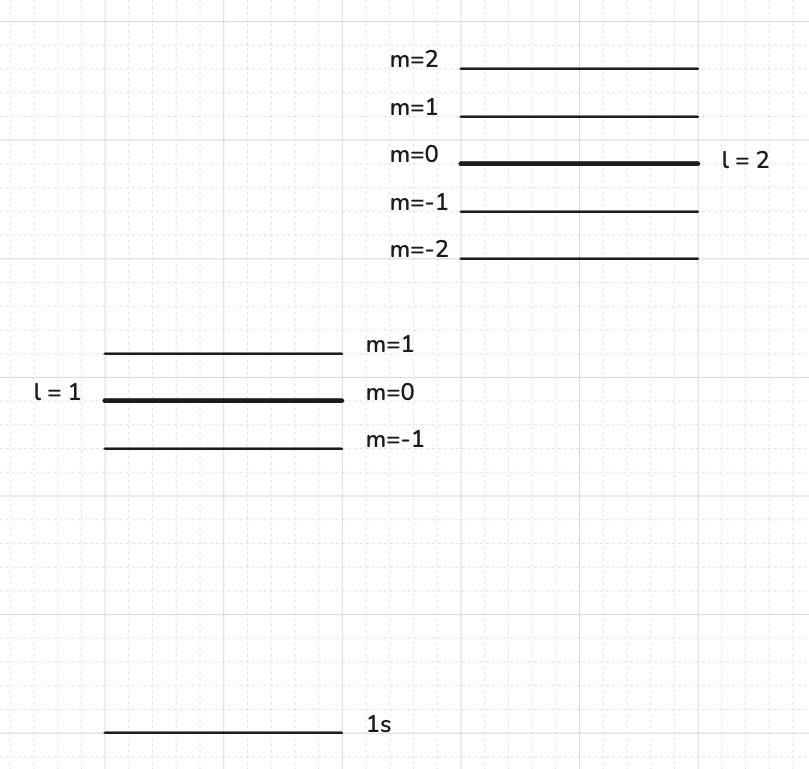
\includegraphics[scale=0.35]{ch11-11.28a.png}
\end{center}

\item [\textbf{(b)}] Let us consider the initial level to be $m_i$ and the
final level $m_f$, then we can count the different transitions as follows.\\
If $m_i = 2$ then the possible transitions are
\begin{align*}
    2 - 1 &= 1 \\
    2 - 0 &= 2 \\
    2 - (-1) &= 3
\end{align*}
If $m_i = 1$ then the possible transitions are
\begin{align*}
    1 - 1 &= 0 \\
    1 - 0 &= 1 \text{ (repeated)}\\
    1 - (-1) &= 2 \text{ (repeated)}
\end{align*}
If $m_i = 0$ then the possible transitions are
\begin{align*}
    0 - 1 &= -1 \\
    0 - 0 &= 0 \text{ (repeated)}\\
    0 - (-1) &= 1 \text{ (repeated)}
\end{align*}
If $m_i = -1$ then the possible transitions are
\begin{align*}
    (-1) - 1 &= -2 \\
    (-1) - 0 &= -1 \text{ (repeated)}\\
    (-1) - (-1) &= 0 \text{ (repeated)}
\end{align*}
If $m_i = -2$ then the possible transitions are
\begin{align*}
    (-2) - 1 &= -3 \\
    (-2) - 0 &= -2 \text{ (repeated)}\\
    (-2) - (-1) &= -1 \text{ (repeated)}
\end{align*}
Therefore there are 7 distinct transitions.

\item [\textbf{(c)}] The allowed transitions that satisfy the selection rules
are
\begin{center}
    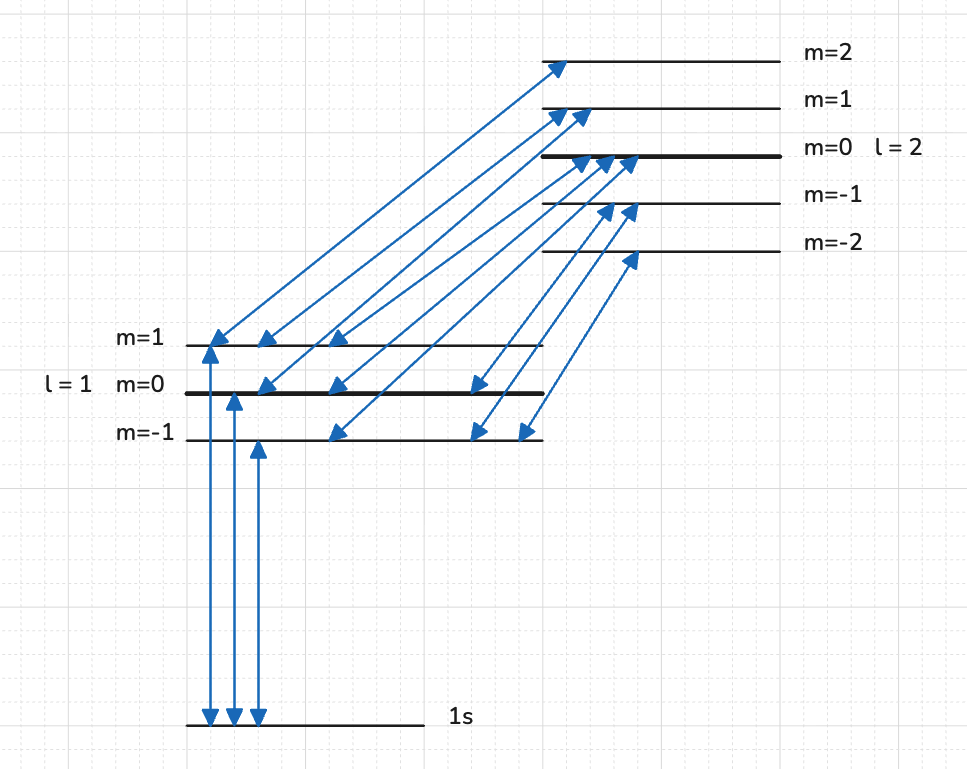
\includegraphics[scale=0.35]{c11-11.28c.png}
\end{center}

\item [\textbf{(d)}] The photon frequencies that will result from the
transitions from the level $l= 1$ to the level $l = 2$ (or viceversa)
depend only on the difference $m_i - m_f$ and since $\Delta m$ can only be 0
or $\pm 1$ then there are only 3 allowed photon frequencies when the electron
transition between the levels $l = 1$ and $l = 2$.\\
Additionally, there are 3 more distinct possible photon frequencies when the
electron transition from the level $l = 1$ to the ground level.\\
Therefore there are 6 distinct photon frequencies.
\end{itemize}
\end{proof}

\cleardoublepage
\begin{proof}{\textbf{11.30}}\\
Equation (8.98) states that the wavefunction is of the form
\begin{align*}
    \psi_{nlm}(r, \theta, \phi) = R_{nl}(r)\Theta_{lm}(\theta) e^{im\phi}
\end{align*}
Let us write the probability integral in spherical coordinates for the $x$
component of the radiation
\begin{align*}
    \int_0^\infty \int_0^\pi \int_0^{2\pi}
    (R_{n'l'}(r)\Theta_{l'm'}(\theta)e^{-im'\phi})
    r\sin\theta\cos\phi
    (R_{nl}(r)\Theta_{lm}(\theta)e^{im\phi})
    ~r^2 \sin\theta dr d\theta d\phi
\end{align*}
For the $\phi$ variable the integral is 
\begin{align*}
    \int_0^{2\pi} \cos\phi e^{-im'\phi} e^{im\phi} ~ d\phi
     = \int_0^{2\pi} \cos\phi e^{i\phi(m-m')} ~ d\phi
\end{align*}
Naming $m - m' = n$ and assuming that $|n| \geq 2$ we get that
\begin{align*}
    \int_0^{2\pi} \cos\phi e^{in\phi} ~ d\phi
    = \frac{i n(1 - e^{2i\pi n})}{n^2 - 1}
\end{align*}
We note that $e^{2i\pi n} = 1$ for $|n| = 2, 3, ...$ so the integral is 0.\\
In the case $n = \pm 1$ i.e. $\Delta m = \pm 1$ we have that 
\begin{align*}
    \int_0^{2\pi} \cos\phi e^{\pm i\phi} ~ d\phi = \pi
\end{align*}
If $\Delta m = 0$ the integral becomes
\begin{align*}
    \int_0^{2\pi} \cos\phi ~ d\phi = 0
\end{align*}
For the $y$ component of the radiation, the $\phi$ integral is
\begin{align*}
    \int_0^{2\pi} \sin\phi e^{i\phi(m-m')} ~ d\phi
\end{align*}
Again, this integral is 0 for any $|\Delta m| =0, 2, 3, ..$ and it's equal to
$i\pi$ for $\Delta m = \pm 1$.
Finally, the $\phi$-intergal for the $z$ component of the radiation is
\begin{align*}
    \int_0^{2\pi} e^{i\phi(m-m')} ~ d\phi
\end{align*}
Which is 0 for $|\Delta m| = 1, 2, 3, ...$ but it's equal to $2\pi$ when
$\Delta m = 0$.\\
Therefore the average of the three integrals is non-zero only when
$\Delta m = 0$ or $\pm 1$.
\end{proof}

\cleardoublepage
\begin{proof}{\textbf{11.31}}
\begin{itemize}
\item [\textbf{(a)}] We know that to interact with the atom, the orbital
angular momentum of the photon must be of order $a_B p$ or less, where $p$ is
the linear momentum of the photon, i.e.
\begin{align*}
    L_\gamma \leq a_B p 
\end{align*}
Then
\begin{align*}
    L_\gamma \leq a_B \frac{E_R}{c} = a_B\frac{ke^2}{2a_Bc}
    = \frac{ke^2\hbar}{2c\hbar} = \frac{\alpha}{2}\hbar \leq \alpha \hbar
\end{align*}
Where we used that $p = E_R/c$, $E_R = ke^2/2a_B$ and that
$\alpha = ke^2/c\hbar$.
\item [\textbf{(b)}] Taking the $z$ component of
$\bm{L'} = \bm{L} + \bm{S}_\gamma$ we see that
\begin{align*}
    L_z' = L_z + S_{\gamma z}
\end{align*}
We know that the maximum value for $L_z$ is $l \hbar$. The allowed values
for $S_{\gamma z}$ are $\hbar, 0, -\hbar$ so $L_z' = l'\hbar$ will be maximum when 
$L_z = l\hbar$ and $S_{\gamma z} = \hbar$ so
\begin{align*}
    l'\hbar &= l\hbar + \hbar \\
    l' &= l + 1
\end{align*}
On the other hand, $L_z'$ will be minimum when $L_z = l\hbar$ and
$S_{\gamma z} = -\hbar$, hence
\begin{align*}
    l' &= l - 1
\end{align*}
Given that the selection rule says that $l' = l$ cannot happen then
$S_{\gamma z} = 0$ is forbidden. Therefore must be that
$\Delta l = l' - l = \pm 1$.
\end{itemize}
\end{proof}

\cleardoublepage
\begin{proof}{\textbf{11.33}}
\begin{itemize}
\item [\textbf{(a)}] We know that the energy of a single photon is
$E = hc/\lambda$, since the laser has $\lambda = 532~nm$ then
$$E = \frac{6.63\sci{-34}~Js\cdot 2.998\sci{8}~m/s}{532\sci{-9}~m}
= 3.736\sci{-19}~J $$
Each pulse has $0.3~J$ then the number of photons sent is
\begin{align*}
    \frac{0.3}{3.736\sci{-19}} = 8.03\sci{17}~\text{photons}
\end{align*}
\item [\textbf{(b)}] The laser beam has a 5 km diameter on the moon so the 
area of the beam is $A_l = \pi 5^2/4 = 19.63~km^2$.\\
The area of each mirror is $\pi (4\sci{-5})^2/4 = 1.25\sci{-9}~km^2$
so the total area of the 300 mirrors is
$A_m = 300 \cdot 1.25\sci{-9} = 3.75\sci{-7}~km^2$.\\
Then the ratio of photons coming back to Earth is
\begin{align*}
    \frac{3.75\sci{-7}}{19.63} = 1.91\sci{-8}
\end{align*}
So the number of photons reaching the Earth would be 
\begin{align*}
    1.91\sci{-8} \cdot 8.03\sci{17}~\text{photons}
    =  15.33\sci{9}~\text{photons}
\end{align*}
\item [\textbf{(c)}] The angular divergence is given by
\begin{align*}
    \delta\theta \approx \frac{\lambda}{d}
    = \frac{532\sci{-9}}{0.04 \cdot 300}
    = 4.43\sci{-8}
\end{align*}
\item [\textbf{(d)}] The diameter of the reflected beam is
\begin{align*}
    d' = 2R = 2L \delta\theta = 2 \cdot 4\sci{8} \cdot 4.43\sci{-8}
    = 35.44~m
\end{align*}
\item [\textbf{(e)}] The area of the beam coming to Earth is 
$\pi d'^2/4 = 986.45~m^2$ and the area of the telescope is
$\pi 1^2/4 = 0.78~m^2$ so the fraction of light captured by the telescope is
\begin{align*}
    \frac{0.78}{986.45} = 0.0008 = 0.08~\%
\end{align*}
\item [\textbf{(f)}] Given that only $0.08~\%$ of the light is captured by the
telescope then the number of photons captured is
\begin{align*}
    15.33\sci{9} \cdot 0.0008 = 12.264\sci{6}~\text{photons}
\end{align*}

\end{itemize}
\end{proof}

\cleardoublepage
\begin{proof}{\textbf{11.34}}\\
Let us consider an infinite square well of width $a = 1$, centered on the
origin and let 
\begin{align*}
    \psi_n(x) = \begin{cases}
        \sqrt{2}\cos n\pi x \qquad (n\text{ is odd}) \\[6pt]
        \sqrt{2}\sin n\pi x \qquad (n\text{ is even})
    \end{cases}
\end{align*}
be the stationary state wave functions. Let also
\begin{align*}
    \psi(x) = \begin{cases}
        1 \qquad  x \in [-1/2, 1/2] \\[6pt]
        0 \qquad  x \in (-\infty, -1/2) \cup (1/2, \infty)
    \end{cases}
\end{align*}
\begin{itemize}
\item [\textbf{(a)}]
Let us compute the coefficients $A_n$ as follows. \\
If $n$ is odd we have that
\begin{align*}
    A_n &= \int_{-\infty}^\infty \psi_n(x)^*\psi(x) ~dx \\
    &= \sqrt{2}\int_{-1/2}^{1/2} \cos n\pi x ~dx \\
    &= \frac{\sqrt{2}}{\pi n}\bigg[\sin n\pi x\bigg]_{-1/2}^{1/2}\\
    &= \frac{\sqrt{2}}{\pi n}
    \bigg[\sin \frac{n\pi}{2} + \sin \frac{n\pi}{2}\bigg]\\
    &= \frac{2\sqrt{2}}{\pi n}\sin \frac{n\pi}{2}
\end{align*}
If $n$ is even then we have that
\begin{align*}
    A_n &= \int_{-\infty}^\infty \psi_n(x)^*\psi(x) ~dx \\
    &= \sqrt{2}\int_{-1/2}^{1/2} \sin n\pi x ~dx \\
    &= -\frac{\sqrt{2}}{\pi n}\bigg[\cos n\pi x\bigg]_{-1/2}^{1/2}\\
    &= -\frac{\sqrt{2}}{\pi n}
    \bigg[\cos \frac{n\pi}{2} - \cos \frac{n\pi}{2}\bigg]\\
    &= 0
\end{align*}

\cleardoublepage
\item [\textbf{(b)}-\textbf{(c)}]
The first 5 nonzero terms of the series are
\begin{align*}
    A_1\psi_1(x) &= \frac{4}{\pi}\cos \pi x &
    A_3\psi_3(x) &= -\frac{4}{3\pi}\cos 3\pi x \\
    A_5\psi_5(x) &= \frac{4}{5\pi}\cos 5\pi x &
    A_7\psi_7(x) &= -\frac{4}{7\pi}\cos 7\pi x \\
    A_9\psi_9(x) &= \frac{4}{9\pi}\cos 9\pi x
\end{align*}
Plotting the sum of the 5 nonzero terms and the 10 nonzero terms we get that
\begin{center}
    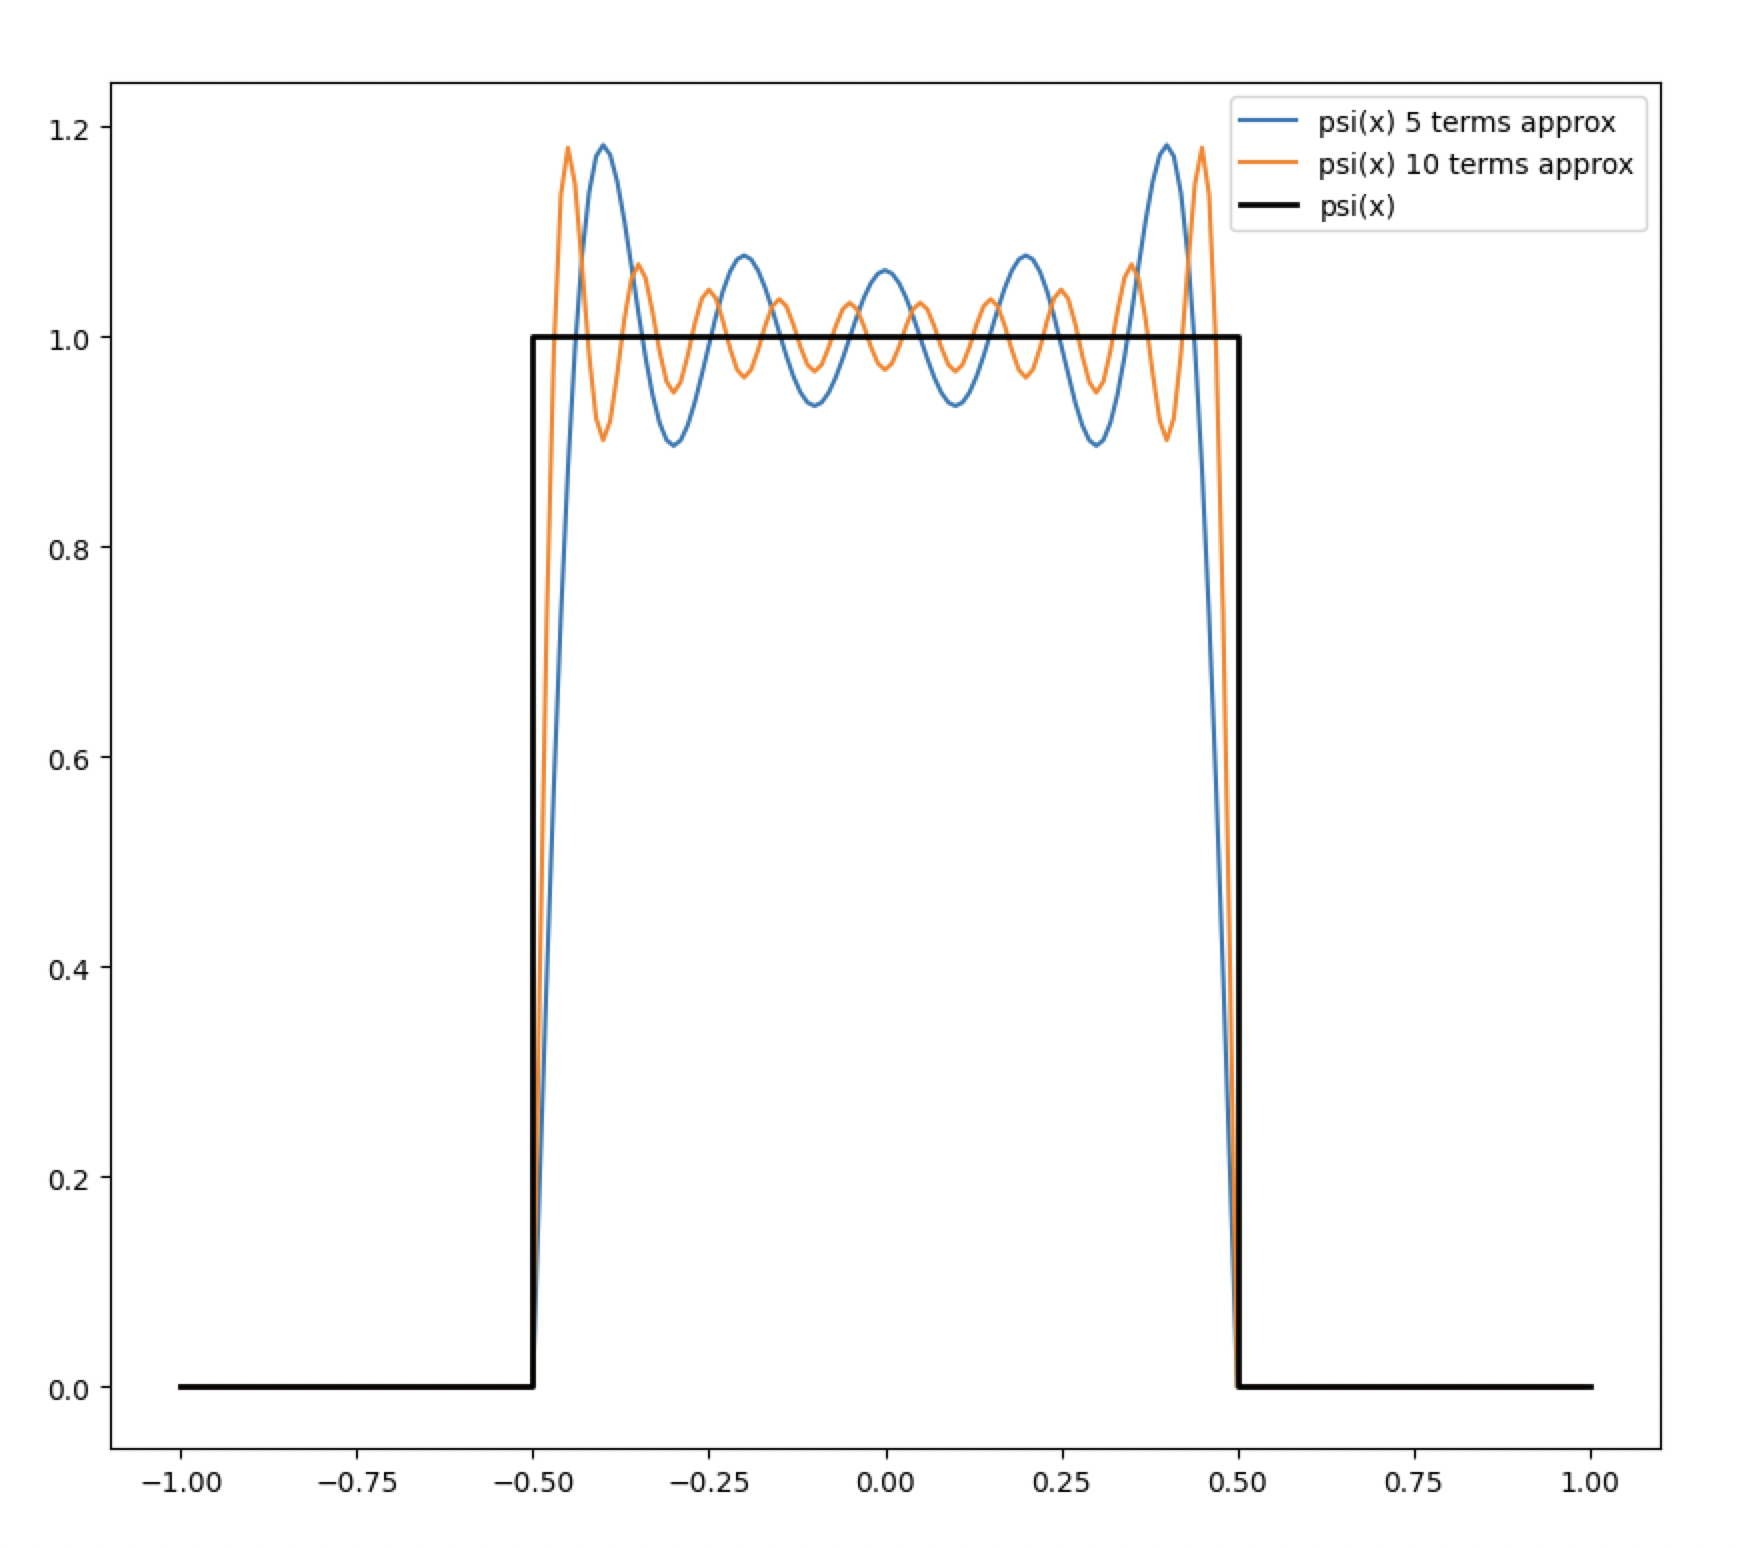
\includegraphics[scale=0.4]{ch11-11.34b-c.png}
\end{center}
\end{itemize}
\end{proof}

\cleardoublepage
\begin{proof}{\textbf{11.35}}\\
Let us consider now
\begin{align*}
    \psi(x) = \sqrt{2}|(1 - 2x)|
\end{align*}
\begin{itemize}
\item [\textbf{(a)}]
Let us compute the coefficients $A_n$ as follows. \\
If $n$ is odd we have that
\begin{align*}
    A_n &= \int_{-\infty}^\infty \psi_n(x)^*\psi(x) ~dx \\
    &= 2\int_{-1/2}^{1/2} (1 - 2x)\cos n\pi x ~dx \\
    &= \frac{4}{\pi n}\sin \frac{n\pi}{2}
\end{align*}
If $n$ is even then we have that
\begin{align*}
    A_n &= \int_{-\infty}^\infty \psi_n(x)^*\psi(x) ~dx \\
    &= 2\int_{-1/2}^{1/2} (1 - 2x)\sin n\pi x ~dx \\
    &= \frac{4}{\pi^2 n^2} \bigg[\pi n\cos\frac{n\pi}{2} - 2\sin \frac{n\pi}{2}\bigg]
\end{align*}

\cleardoublepage
\item [\textbf{(b)}-\textbf{(c)}]
Plotting the sum of the 5 nonzero terms and the 10 nonzero terms we get that
\begin{center}
    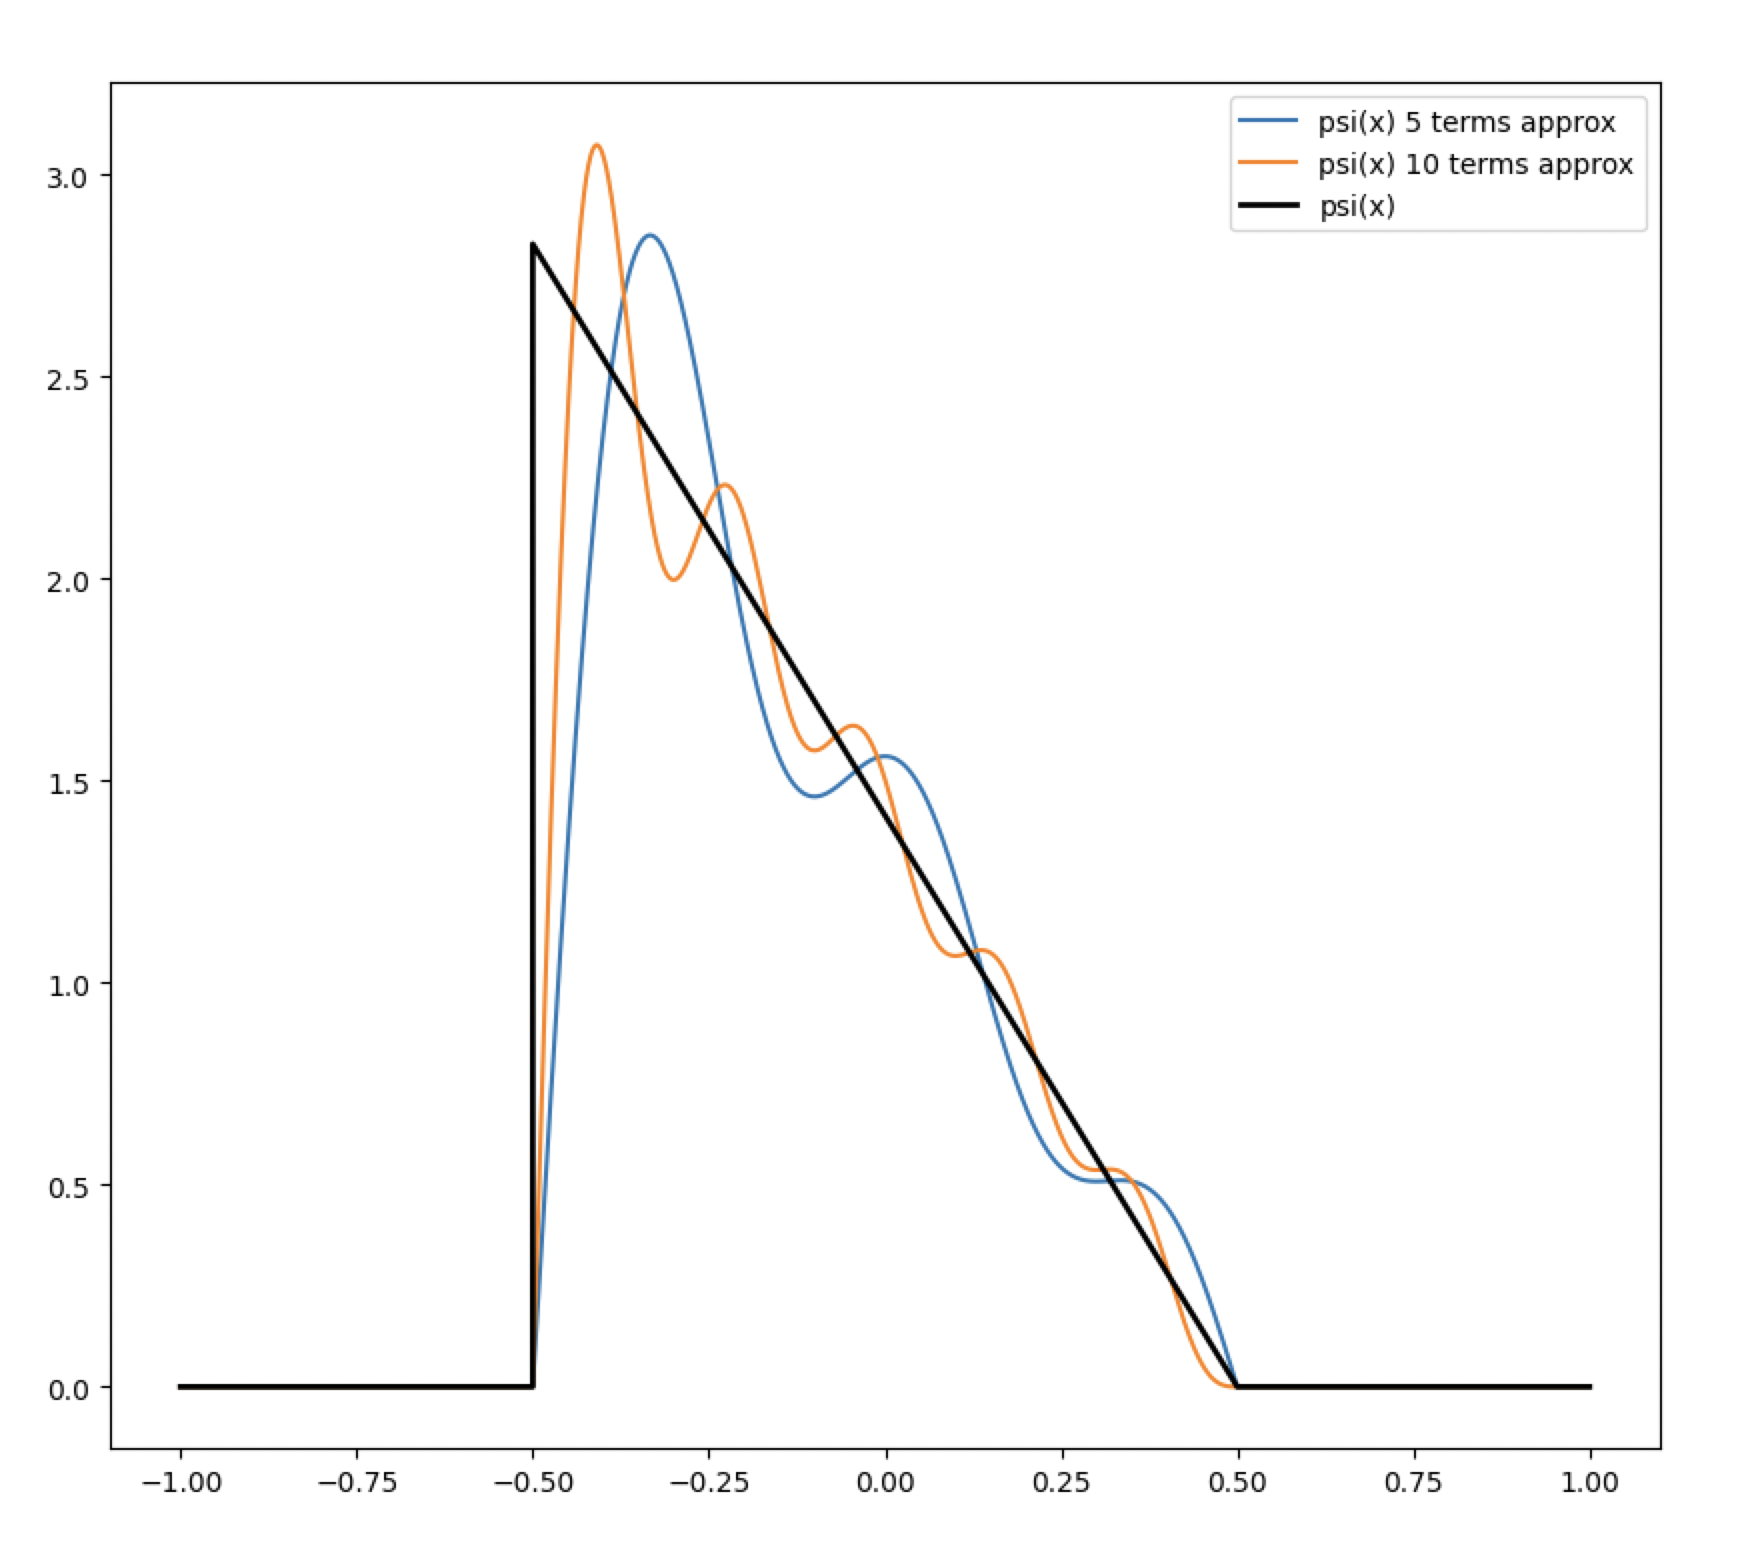
\includegraphics[scale=0.4]{ch11-11.35b-c.png}
\end{center}
\end{itemize}
\end{proof}

\cleardoublepage
\begin{proof}{\textbf{11.36}}\\
\begin{itemize}
\item [\textbf{(a)}] Below we plot $\psi_2(x)$ and $x\psi_2(x)$ assuming
$a = 1$.
\begin{center}
    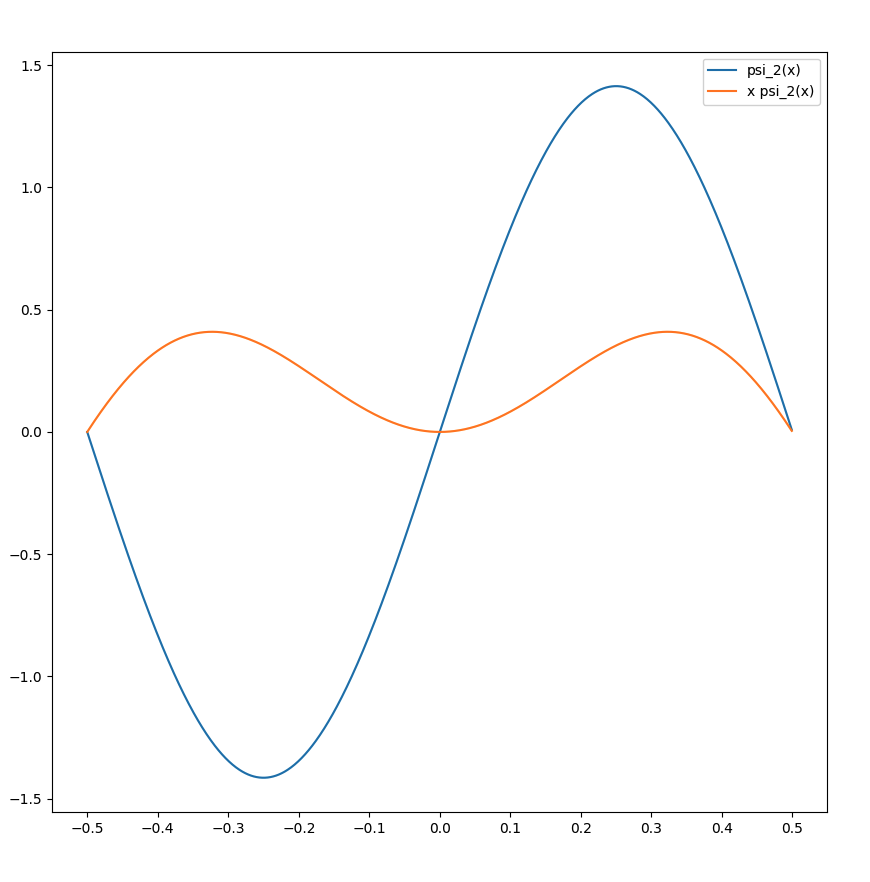
\includegraphics[scale=0.35]{ch11-11.36a.png}
\end{center}
\item [\textbf{(b)}] Let us expand the function $x\psi_2(x)$, then the
coefficients $A_n$ if $n$ is odd are given by
\begin{align*}
    A_n &= \int_{-\infty}^\infty \psi_n(x)^* x\psi_2(x)~dx\\
    &= \frac{2}{a}\int_{-a/2}^{a/2}
    x\cos\frac{n\pi x}{a}\sin\frac{2\pi x}{a}~dx\\
    &= -\frac{4a[\pi(n^2 - 4)\cos(n\pi/2) - 4n\sin(n\pi/2)]}{\pi^2(n -2)^2(n +2)^2}
\end{align*}
If $n$ is even
\begin{align*}
    A_n &= \frac{2}{a}\int_{-a/2}^{a/2}
    x\sin\frac{n\pi x}{a}\sin\frac{2\pi x}{a}~dx
    = 0
\end{align*}
Therefore to a good extent we can approximate $x\psi_2(x)$ as
\begin{align*}
    x\psi_2(x) &\approx A_1\psi_1(x) + A_3\psi_3(x) \\
    &= \frac{4a[3\pi\cos(\pi/2) + 4\sin(\pi/2)]}{9\pi^2}\psi_1(x) \\
    &\quad-\frac{4a[5\pi\cos(3\pi/2) - 12\sin(3\pi/2)]}{25\pi^2}\psi_3(x) \\
    &= \frac{16a}{9\pi^2}\psi_1(x) - \frac{48a}{25\pi^2}\psi_3(x) \\
    &= \sqrt{2/a}\bigg[\frac{16a}{9\pi^2}\cos\frac{\pi x}{a}
    - \frac{48a}{25\pi^2}\cos\frac{3 \pi x}{a}\bigg]
\end{align*}
If we assume $a = 1$ we can plot the approximation against the real value as
follows
\begin{center}
    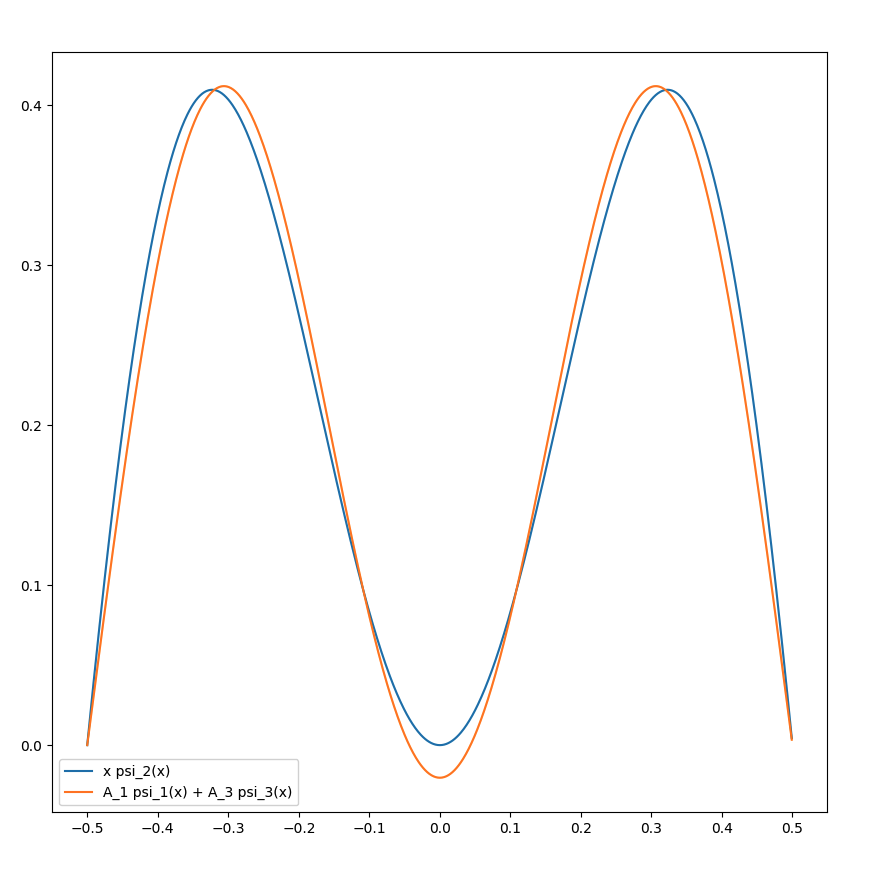
\includegraphics[scale=0.35]{ch11-11.36b.png}
\end{center}
The physical significance of this is that adding a perturbation to the state
$\psi_2$ adds a term to the wave function that closely approximates
$A\psi_1 + B\psi_3$.
\end{itemize}
\end{proof}
\end{document}

